\documentclass{nitk}
\usepackage{fullpage}
% \usepackage{geometry}
\usepackage{tabularx}
\usepackage{amssymb}
\usepackage{amsmath}
\usepackage{array}
\usepackage{appendix}
\usepackage{enumerate}
\usepackage{subcaption}
\usepackage[english]{babel}
\usepackage[utf8]{inputenc}
\usepackage{algorithm}
\usepackage[noend]{algpseudocode}
\usepackage[numbers, sort, comma, square]{natbib}
% \usepackage[ruled,novlined,linesnumbered,noresetcount]{algorithm2e}
\newcommand\norm[1]{\left\lVert#1\right\rVert}
% The document class to be used is nitk.
% Internally, it is an extension of the LaTeX article class.

\report{Major Project Progress Report} % What report is this?
\title{Neural Networks For Image Analysis} % What is the title of the report?
% \rollno{14IT103}
\author{
    Siddhanth Pillay \\
    15IT129
}
\guidea{Dr Sowmya Kamath S} % Who is the guide? Or who are you submitting this work to?
\guideb{Dr. Suyash Awate (IITB)}
\dept{Dept. of Information Technology} % What is the department you are submitting the report to?
\years{December 2018}
\place{Surathkal} % The place to be used in the declaration.

\begin{document}
    \maketitle % Builds the first page in NITK Template format.
    \newpage
    \thispagestyle{empty}
    \begin{tikzpicture}[remember picture, overlay]%
        \draw[line width = 1pt] ($(current page.north west) + (2em,-2em)$) rectangle ($(current page.south east) + (-2em,2em)$);%
    \end{tikzpicture}%
    \begin{center}
        {\Large \textbf{Department of Information Technology}}\\
        {\large \textbf{National Institute of Technology Karnataka, Surathkal}}\\
      \vspace{20}
        {\large \underline {\textbf{Project Progress Evaluation}}}
    \end{center}
    \vspace{10}
    \begin{flushleft}
    {\large \textit{Course Code:} {IT 499}}
    \vspace{15}
    \\
    {\large \textit{Course Title:} {Major Project II}}
    \vspace{15}
    \\
    {\large \textit{Title of the Project:} {Neural  Networks For Image Analysis}}
    \vspace{15}
    \\
    {\large \textit{Details of Project Group}}
    \vspace{15}
    \\
    {\large \textit{Name of the student}} \hspace{30} {\large \textit{Register No.}} \hspace{50} {\large \textit{Signature with date}}
    % \begin{tabularx}{\textwidth}{XXX}
    % {\large \textit{Name of the student}} & {\large \textit{Register No.}} & {\large \textit{Signature with date}}
    % \end{tabularx}
    \hline
    \vspace{10}
    {1. Siddhanth Pillay\hspace{70}15IT129}\\\vspace{10}
    \vspace{10}
    \vfill
     {\large \textbf{Name of Project Guide: Dr.Sowmya Kamath S}}
    \vspace{15}
    \\
     {\large \text{Signature of Project Guide:}}
    \vspace{15}
    \\
     {\large \text{Place: NITK Surathkal}}
    \vspace{15}
    \\
     {\large \text{Date: 25 March 2019}}
    \vspace{15}
    \\
    \end{flushleft}
    % \abstract{My topic is  blah blah} % Write abstract within the \abstract{} command.
    \newpage
    % \makedeclaration 
    \abstract {
    
    \hspace{20} The count of White Blood Cells in a Blood Sample can provide a plethora of information about the state of one's immune system and any potential risks that one could be facing. Understanding the count of one's White Blood Cells(WBCs) can offer a powerful quantitative picture of one's health. The automated way of counting WBCs requires the use of expensive tools, whereas the manual way is very time-consuming and based on extrapolation, which brings with it a certain error rate. Deep Learning methods provide a promising advancement for this task, because it is cheap, takes lesser time, and improves its performance over time. Hence, a Neural Network based sliding-window approach for the task of counting White Blood Cells in a Blood Sample is proposed. The model demonstrates near-perfect accuracy in counting the White Blood Cells and also shows very good results in identifying other objects like Red Blood Cells and Platelets. By comparing the model with a powerful baseline of an Autoencoder and Support Vector Machine, the power and efficiency of the model is demonstrated. 
    
    }
    \tableofcontents
    \listoffigures
    % \listoftables
    
    \pagenumbering{arabic} % This is needed so that the body of the report has numbering starting from 1.
    \section{Introduction} % Begin body of the report.
     
    Some of the more popular statistics that doctors look for when they take a blood sample are as follows:
    \begin{itemize}
        \item Total number of White Blood Cells (WBCs) in the blood stream
        \item The number of Neutrophils, Lymphocytes, Basophils, and Eosinophils (all types of WBCs) in the blood sample. This is known as a differentiated blood cell count.
    \end{itemize}
    
    The density of WBCs in the blood stream provides a glimpse into the state of one's immune system and any potential risks one might be facing. In particular, a dramatic change in the WBC count relative to the baseline is generally a sign that the body is currently being affected by an antigen. Moreover, a variation in a specific type of WBC generally correlates with a specific type of antigen. For instance, Leukemia patients often see a dramatically higher level of Lymphocytes in their blood stream relative due to a malfunctioning immune system. Likewise, people fighting allergies generally see an increase in their Eosinophil counts as these WBCs are key to fighting allergens. As such, understanding the count of White Blood Cells in one's blood stream can provide us a powerful quantitative picture of one's health. \\ \par
    
    {Neural Networks offer a glimpse into the manner in which the process of human learning can be converted into an algorithm. Neural Networks offer a lot of advantages in over other learning algorithms. Neural networks have the capability of optimising the relationship between the inputs and outputs via distributed computing, training, and processing, leading to reliable solutions desired by specifications. Neural networks have the nature of adaptive learning from input information and, using a suitable learning algorithm, can improve themselves in accordance with the variety and the change of input content. Neural Networks are also called as ``Universal Function Approximators" because of their ability to approximate any function given a sufficient amount of data. \\}
    
    {Thus, Neural Networks are powerful tools that can be utilised to automate the process of detecting White Blood Cells in Blood Samples. Hence, a Neural Network based model for performing semantic segmentation of Neural Networks is proposed. By comparing this model with other powerful baselines, the efficiency of the model is demonstrated. \\}
    
    \subsection{Motivation}
    
    There are two main ways the different types of WBCs in blood streams are counted: the automated way and the manual way. \\ \par
    
    The earliest automated way uses a device invented in the 1950s known as a Coulter Counter. At a high level, a Coulter Counter uses the fact that WBCs are poor conductors of electricity to classify and count them. More recently, Laser Flow Cytometers have emerged as an improved alternative to Coulter Counters. These devices shine a laser across a channel and measure how the light from the laser is refracted as cells pass through. Based on the refraction of light, the device aims to classify the given cell. However, both Coulter Counters and Laser Flow Cytometers cost in tens of thousands of dollars. This makes it inaccessible for many patients all over the world. \\ \par
    
    In the manual approach, a sample of blood is placed under a microscope and a pathologist manually counts the number of cells in each frame. The total count is then extrapolated by assuming that the distribution is uniform across the entire blood sample and multiplying up. \\ \par
    
    The Deep Learning based approach proposed in this work is a potentially promising advancement over such techniques due to the following reasons:
    \begin{itemize}
        \item It requires far cheaper equipment thanks to being reliant on simple imaging.
        \item It requires significantly lesser time to provide results as compared to the previously stated methods
        \item It promises to get better over time as classification and counting of more and more blood cells is performed to increase the size of the dataset. It can be continously updated to provide continously improving results. 
        \item It offers a low-cost solution to performing a task that was otherwise tedious and expensive, which can be used in low-income regions that do not have significant healthcare facilities. 
    \end{itemize}
    
    \pagebreak 
    \section{Related Work}
    \par
    The task of segmentation is typically defined as identifying the set of voxels which make up either the contour or the interior of the object(s) of interest. Segmentation is the most common subject of papers applying deep learning to medical imaging, and as such has also seen the widest variety in methodology, including the development of unique CNN-based segmentation architectures and the wider application of RNNs. \\ \par
    
    The most well-known, in medical image analysis, of these
novel CNN architectures is U-net, published by \citet{ronneberger2015u}. The two main architectural novelties in U- net are the combination of an equal amount of upsampling and downsampling layers. Although learned upsampling layers have been proposed before, U-net combines them with so-called skip connections between opposing convolution and deconvolution layers. This which concatenate features from the contracting and expanding paths. From a training perspective this means that entire images/scans can be processed by U-net in one forward pass, resulting in a segmentation map directly. This allows U-net to take into account the full context of the image, which can be an advantage in contrast to patch-based CNNs. Furthermore, in an extended paper by \citet{cciccek20163d} , it is shown that a full 3D segmentation can be achieved by feeding U-net with a few 2D annotated slices from the same volume. Other authors have also built derivatives of the U-net architecture; \citet{milletari2016v}, for example, proposed a 3D-variant of U-net architecture, called V-net, performing 3D image segmentation using 3D convolutional layers with an objective function directly based on the Dice coefficient. \citet{drozdzal2016importance} investigated the use of short ResNet-like skip connections in addition to the long skip-connections in a regular U-net. \\ \par

RNNs have recently become more popular for segmentation
tasks. For example, \citet{xie2016spatial} used a spatial clockwork RNN to segment the perimysium in H&E-histopathology images. This network takes into account prior information from both the row and column predecessors of the current patch. To incorporate bidirectional information from both left/top and right/bottom neighbors, the RNN is applied four times in different orientations and the end-result is concatenated and fed to a fully-connected layer. This produces the final output for a single patch. \citet{stollenga2015parallel} where the first to use a 3D LSTM-RNN with convolutional layers in six directions. \citet{andermatt2016multi} used a 3D RNN with gated recurrent units to segment gray and white matter in a brain MRI data set. \citet{chen2016dcan} combined bi-directional LSTM-RNNs with 2D U-net-like-architectures to segment structures in anisotropic 3D electron microscopy images. Last, \citet{poudel2016recurrent} combined a 2D U-net architecture with a gated recurrent unit to perform 3D segmentation. \\ \par

Although these specific segmentation architectures offered
compelling advantages, many authors have also obtained excellent segmentation results with patch-trained neural networks. One of the earliest papers covering medical image segmentation with deep learning algorithms used such a strategy and was published by \citet{ciresan2012deep} . They applied pixel-wise segmentation of membranes in electron microscopy imagery in a sliding window fashion. Most recent papers now use fCNNs in preference over sliding-window-based classification to reduce redundant computation. \\ \par

fCNNs have also been extended to 3D and have been applied to multiple targets at once: \citet{korez2016model}, used 3D fCNNs to generate vertebral body likelihood maps which drove deformable models for vertebral body segmentation in MR images, \citet{zhou2016three} segmented nineteen targets in the human torso, and \citet{moeskops2016deep} trained a single fCNN to segment brain MRI, the pectoral muscle in breast MRI, and the coronary arteries in cardiac CT angiography (CTA). \\ \par

One challenge with voxel classification approaches is that they sometimes lead to spurious responses. To combat this, groups have tried to combine fCNNs with graphical models like MRFs ( \citet{shakeri2016sub}; \citet{song2015accurate} ) and Conditional Random Fields (CRFs) ( \citet{alansary2016fast}; \citet{cai2017pancreas}; \citet{christ2016automatic}; \citet{dou2016automatic}; \citet{fu2016deepvessel}; \citet{gao2016segmentation} ) to refine the segmentation output. In most of the cases, graphical models are applied on top of the likelihood map produced by CNNs or fCNNs and act as label regularizers. \\ \par

Summarizing, segmentation in medical imaging has seen a huge
influx of deep learning related methods. Custom architectures have been created to directly target the segmentation task. These have obtained promising results, rivaling and often improving over results obtained with fCNNs. \\ \par

Segmentation of lesions combines the challenges of object detection and organ and substructure segmentation in the application of deep learning algorithms. Global and local context are typically needed to perform accurate segmentation, such that multi-stream networks with different scales or non-uniformly sampled patches are used as in for example \citet{kamnitsas2017efficient} and \citet{ghafoorian2016non} . In lesion segmentation, we have also seen the application of U-net and similar architectures to leverage both this global and local context. The architecture used by \citet{wang2015unified}, similar to the U-net, consists of the same downsampling and upsampling paths, but does not use skip connections. Another U-net-like architecture was used by \citet{brosch2016deep} to segment white matter lesions in brain MRI. However, they used 3D convolutions and a single skip connection between the first convolutional and last deconvolutional layers.\\ \par

One other challenge that lesion segmentation shares with object detection is class imbalance, as most voxels/pixels in an image are from the non-diseased class. Some papers combat this by adapting the loss function: \citet{brosch2016deep} defined it to be a weighted combination of the sensitivity and the specificity, with a larger weight for the specificity to make it less sensitive to the data imbalance. Others balance the data set by performing data augmentation on positive samples ( \citet{kamnitsas2017efficient}; \citet{litjens2016deep}; \citet{pereira2016brain} ). \\ \par

Thus lesion segmentation sees a mixture of approaches used in
object detection and organ segmentation. Developments in these two areas will most likely naturally propagate to lesion segmentation as the existing challenges are also mostly similar.
    
    \subsection{Outcome of Literature Review}
    {\hspace{20}In this section the considered research papers are analyzed based on the fulfillment of a selection of important criteria. In order to group and compare the research work appropriately, the criteria include general aspects, e.g., the base technology of the work, as well as specific topics tackled by the authors. The selected criteria for the classification of the related work are the following.
    
    \begin{enumerate}
    \item{\textbf{Class Imbalance}\\
    From the literature survey, it became apparent that in almost every semantic segmentation task, there is a dominance of the non-diseased class. This poses a problem while training, because one needs to balance out the two classes in order to get optimally trained models. Different approaches were proposed to tackle this problem, such as adapting the loss function, balancing the dataset by augmenting the positive samples, etc.}
    
    \item{\textbf{Specificity of the Models} \\
    From the literature survey, one can notice that there are a lot of successful models that are built specifically for a particular task/dataset. There are very few models that can be applied `in general' to different datasets. This stands in contrast to the other applications of Deep Learning, such as Image Captioning, Object Classification, etc., where we see the cross-applicability of models. Hence, there is the need of the development of a universal model that can give accurate results on different datasets. 
    }
    \end{enumerate}
    
    }
    
    \subsection{Problem Statement}
    {\hspace{20} To develop a sliding-window based Neural Network approach to performing Semantic Segmentation of Malaria Cells in Thin Blood Films}
    
    \subsection{Research Objectives}
    
    {\hspace{20} The objective of the project is to develop a sliding-window based Neural Network approach to performing Semantic Segmentation on Microscopy Images of Blood Samples. This study also aims at demonstrating the efficacy of the model by comparing the results with a powerful baseline. The tasks to be performed to realize the objective are as follows:\\
    
    \begin{itemize}
        \item Develop a training balanced dataset to categorise between the infected cells and non-infected regions
        \item Develop a sliding window approach to make the classifier work on every pixel of the entire image
        \item Select a simple Neural Network Image Classification Model with a simple yet powerful architecture to give accurate segmentation results
        \item Select a powerful baseline to compare the results with the Neural Network Classifier and demonstrate the efficacy of the model
    \end{itemize}
   \\
   }
    \pagebreak
    
    \section{Methodology}

\subsection{Reinhard\cite{reinhard2001color} Staining Method}

In this method, Reinhard et al\cite{reinhard2001color} develop a method of applying the colors of one image to another. In order to simplify the process of color transformation, they first convert the color space from RGB to $l\alpha\beta$. 

\begin{equation}
    \begin{pmatrix} L \\ M \\ S \end{pmatrix} = 
    \begin{pmatrix} 0.3811 & 0.5783 & 0.0402 \\ 0.1967 & 0.7244 & 0.0782 \\ 0.0241 & 0.1288 & 0.8444 \end{pmatrix}
    \begin{pmatrix} R \\ G \\ B \end{pmatrix}
\end{equation}

In order to eliminate the large amount of skew present in this color space, logarithm operation is performed:

\begin{equation}
\begin{array}{l}
L = log(L) \\
% \end{equation}

% \begin{equation}
    M = log(M) \\
% \end{equation}

% \begin{equation}
    S = log(S) \\
\end{array}
\end{equation}

\begin{equation}
    \begin{pmatrix} l \\ \alpha \\ \beta \end{pmatrix} = 
    \begin{pmatrix} \frac{1}{\sqrt{3}} & 0 & 0 \\ 0 & \frac{1}{\sqrt{6}} & 0 \\ 0 & 0 & \frac{1}{\sqrt{2}} \end{pmatrix}
    \begin{pmatrix} 1 & 1 & 1 \\ 1 & 1 & -2 \\ 1 & -1 & 0 \end{pmatrix}
    \begin{pmatrix} L \\ M \\ S \end{pmatrix}
\end{equation}

They then perform mean normalization across each of these axes independently:

\begin{equation}
    \begin{array}{l}
         l^{*} = l - \langle l \rangle \\
         \alpha^{*} = \alpha - \langle \alpha \rangle \\
         \beta^{*} = \beta - \langle \beta \rangle \\
    \end{array}
\end{equation}

The mean normalized values are then scaled independently by using the standard deviations of the source and target images:

% and then scale the axes using the standard deviations of the source and target images.  The different equations are as follows:

\begin{equation}
    \begin{array}{l}
    l^{'} = \frac{\sigma_{t}^{l}}{\sigma_{s}^{l}}l^{*} \\
    \alpha^{'} = \frac{\sigma_{t}^{\alpha}}{\sigma_{s}^{\alpha}}\alpha^{*} \\
    \beta^{'} = \frac{\sigma_{t}^{\beta}}{\sigma_{s}^{\beta}}\beta^{*} \\
    \end{array}
\end{equation}
    
In order to invert the transformed images from the $l\alpha\beta$ space to RGB space, first the mean values of the target images (not the source image) are added. Then the inversion process is performed by using the following equations:    
    
\begin{equation}
    \begin{pmatrix} L \\ M \\ S \end{pmatrix} =
    \begin{pmatrix} 1 & 1 & 1 \\ 1 & 1 & -1 \\ 1 & -2 & 0 \end{pmatrix}
    \begin{pmatrix} \frac{1}{\sqrt{3}} & 0 & 0 \\ 0 & \frac{1}{\sqrt{6}} & 0 \\ 0 & 0 & \frac{1}{\sqrt{2}} \end{pmatrix}
    \begin{pmatrix} l \\ \alpha \\ \beta \end{pmatrix}
\end{equation}

\begin{equation}
    \begin{pmatrix} R \\ G \\ B \end{pmatrix} = 
    \begin{pmatrix} 4.4679 & -3.5873 & 0.1193 \\ -1.2186 & 2.3809 & -0.1624 \\ 0.0497 & -0.2439 & 1.2045 \end{pmatrix}
    \begin{pmatrix} L \\ M \\ S \end{pmatrix}
\end{equation}

\subsection{Macenko\cite{macenko2009method} Staining Method}

In this work\cite{macenko2009method}, the assumption is that there is a specific stain vector corresponding to each of the two stains present in the image, and that the resulting color (in OD space) of every pixel is a linear combination of these stain vectors. Since there has to be a non-negative weight on each component, every value must exist between the two stain vectors. If noise were not a factor, the minimum and maximum along the found direction would be used. Instead, robust versions of the minimum and maximum are used by taking the $\alpha$th and ($100-\alpha$)th percentile. Empirically, $\alpha$ = 1 provides robust results.

\begin{algorithm}
\caption{Macenko Staining Method}
\begin{algorithmic}[1]
\State Convert RGB to OD
\State Remove data with OD intensity less than $\beta$
\State Calculate SVD on the OD tuples
\State Create plane from the SVD directions corresponding to the two largest singular values
\State Project data onto the plane, and normaliz to unit length
\State Calculate angle of each point wrt the first SVD Direction
\State Find robust extremes $(\alpha^{th} and (100-\alpha)^{th} percentiles)$ of the angle
\State Convert extreme values back to OD space
\end{algorithmic}
\end{algorithm}

\subsection{Algorithm}

The approach basically consists of a sliding-window or a patch-based approach. The algorithm essentially consists of the following steps:

\begin{enumerate}
    \item Apply the Stain Normalization Technique on the original input image
    \item Select a patch of the image around a given pixel
    \item Pass the patch through the classifier model for pixel-wise classification
    \item Repeat the same process iteratively for all the pixels in the image
\end{enumerate}

One may notice that depending on the size of the patch, a certain number of pixels at the border regions may be left out. This is a valid concern, but it is accounted for by the fact that in the images, none of the Objects of Interest are present at the border regions. Further, the classifications obtained at the borders can be extended to accomodate the size of the entire image. 

\subsection{Base Classifier Architecture}    
    In this experiment, LeNet was chosen as the Convolutional Neural Network architecture. LeNet is composed of 7 layers(not counting the input), all of which contain the trainable parameters (weights). The input to the network is the image of a patch of size 80x80. In the following description, convolutional layers are labeled Cx, subsampling layers are labeled Sx, and fully-convolutional layers are labeled Fx, where x is the index of the layer. \\ \par

Layer C1 is a convolutional layer with 6 feature maps. Each unit in each feature map is connected to a 5x5 neighborhood in the input. The size of the feature maps is 76x76. C1 contains 156 trainable parameters.  \\ \par

Layer S2 is a subsampling layer with 6 feature maps. Each unit in each feature map is connected to a 2x2 neighborhood in the corresponding feature map in C1. The four inputs to a unit in S2 are passed through a max function to select the maximum among these values. The 2x2 receptive fields are non-overlapping, therefore feature maps in S2 have half the number of rows and columns as feature maps in C1. Layer S2 has no trainable parameters. \\ \par

Layer C3 is a convolutional layer that has 16 feature maps. Each unit in each feature map is connected to several 5x5 neighborhoods at identical locations in a subset of S2's feature maps. Layer C3 has 1516 trainable parameters. \\ \par

Layer S4 is a subsampling layer with 16 feature maps. Each unit in each feature map is connected to a 2x2 neighborhood in the corresponding feature map in C3, in a similar way as in C1 and S2. Layer S4 has no trainable parameters. \\ \par

The feature maps obtained from S4 are then arranged in a vector form. Each unit in the vector is connected to each node in the Layer C5. Thus, this forms a fully connected layer. The total number of nodes in the layer C5 is 120. \\ \par

Layer F6 has 84 units and is fully connected to C5. It has 10,164 trainable connections. \\ \par

Finally, the units in F6 layer are fully connected to output layer which contains 2 nodes (one for each class). The values of the output layer are passed through a softmax function to give us the probability values for each of the class. \\ \par

The ReLU activation function is used after performing computations at layers C1, C3, C5 and F6.

\begin{figure}
        \centering
        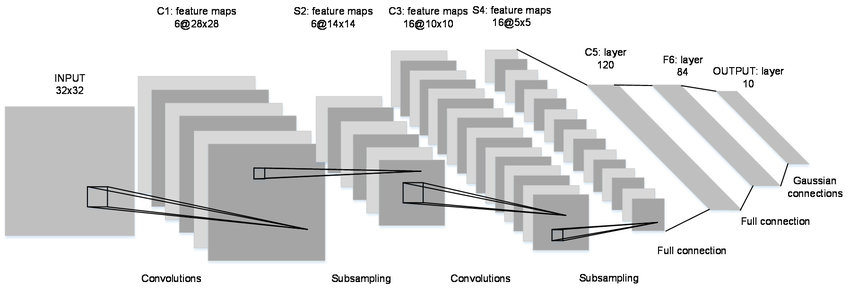
\includegraphics[width=\linewidth]{images/LeNet.png}
        \caption{LeNet Model}
        \label{LeNet}
\end{figure}
    
\newpage
\section{Work Done and Results}
    
We noticed that the dataset provided had a lot of variations in terms of the contrast of the stain color with the background, background light and stain `noise'. Hence, we first filter the images to select those ones which have significant contrast difference between the infected cells and normal cells which are stained. As a data preprocessing step, we applied stain normalization techniques as defined in \cite{macenko2009method}, \cite{reinhard2001color} and \cite{} separately. Then for training the model, we created patch images for each of the classes. For Malaria patches, we calculated the mid-point of the bounding boxes provided in the annotation and created a 80x80 patch around the mid-point. For the non-malaria patches, we selected pixels randomly from the non-infected regions of the image and took an 80x80 patch. This step is then repeated for all the images in the dataset. Consequently, 1502 malaria images and 1502 non-malaria images were obtained as a training set.  \\ \par

The LeNet model is then trained over this dataset by using Cross Entropy Loss and Stochastic Gradient Descent Optimization with default parameters for 50 epochs. For obtaining the pixel-level classification images, we iterate over all the pixels in the entire image and at each pixel, collect values of the pixels falling around the pixel in the defined patch size of 80x80. This patch is then passed through the LeNet model and the label with the maximum value is chosen as the pixel label. \\ \par

We noticed that there were a lot of small-sized false positives that were being generated. Hence, in order to eliminate those, an area threshold was applied. If a particular patch detection crosses the area threshold applied, only then it is considered as a positive detection. We varied the sizes of the area threshold and analysed the performance for each of the staining methods used. The results are shown in Tables \ref{tab:macenko}, \ref{tab:reinhard}, \ref{tab:vahadane}. \\ \par

From Tables \ref{tab:macenko}, \ref{tab:reinhard} and \ref{tab:vahadane}, we can see that the results obtained by the Vahadane et al\cite{} method is the most robust to false positive noise. It also performs the best under the application of area threshold values. The results of Reinhard et al\cite{reinhard} stand in constrast to this since they perform the worst under the application of the area threshold. 

\begin{table}[]
    \centering
    \begin{tabular}{c|c|c|c}
         Area Threshold & True Positives & False Positives & False Negatives  \\
         \hline
         0 & 116 & 4072 & 10 \\
         100 & 116 & 2525 & 10 \\
         200 & 116 & 1831 & 10 \\
         300 & 115 & 1445 & 11 \\
         400 & 115 & 1197 & 11 \\
         500 & 115 & 1049 & 11 \\
         600 & 115 & 939 & 11 \\
         700 & 115 & 863 & 11 \\
         800 & 115 & 823 & 11 \\
         900 & 115 & 785 & 11 \\
         1600 & 112 & 653 & 14 \\
         2500 & 111 & 551 & 15 \\
         3600 & 109 & 468 & 17 \\
         4900 & 106 & 389 & 20
    \end{tabular}
    \caption{Macenko\cite{macenko2009method} Staining}
    \label{tab:macenko}
\end{table}

\begin{table}[]
    \centering
    \begin{tabular}{c|c|c|c}
         Area Threshold & True Positives & False Positives & False Negatives  \\
         \hline
         0 & 109 & 2233 & 18 \\
100	& 109 &	1379 &	18 \\
200	& 107 &	1008 &	20 \\
300	& 106 &	784 &	21 \\
400	& 106 &	620	& 21 \\
500	& 105 &	508 &	22 \\
600	& 105 &	456 &	22 \\
700	& 104 &	406 &	23 \\
800	& 103 & 388	& 24 \\
900	& 101 &	362 &	26 \\
1600 &	98 &	274 &	28 \\
2500 &	89 &	197 &	37 \\
3600 &	83 &	154 &	43 \\
4900 &	74 &	107 & 	52 \\
    \end{tabular}
    \caption{Reinhard\cite{reinhard2001color} Staining}
    \label{tab:reinhard}
\end{table}

\begin{table}[]
    \centering
    \begin{tabular}{c|c|c|c}
         Area Threshold & True Positives & False Positives & False Negatives  \\
         \hline
         0 &	116 &	3220 &	10 \\
100	& 116 &	1507 &	10 \\
200	& 116 & 1079 &	10 \\
300	& 115 &	857 &	11 \\
400	& 115 &	719 &	11 \\
500	& 115 &	626 &	11 \\
600	& 115 &	569 &	11 \\
700	& 115 &	515	& 11 \\
800	& 115 &	493 &	11 \\
900	& 115 &	469 &	11 \\
1600 &	114 &	384 &	12 \\
2500 &	114 &	340 &	12 \\
3600 &	111 &	304 &	15 \\
4900 &	109 &	255 &	17 
    \end{tabular}
    \caption{Vahadane\cite{} Staining}
    \label{tab:vahadane}
\end{table}

\begin{figure}
    \centering
    \begin{subfigure}{0.3\textwidth}
    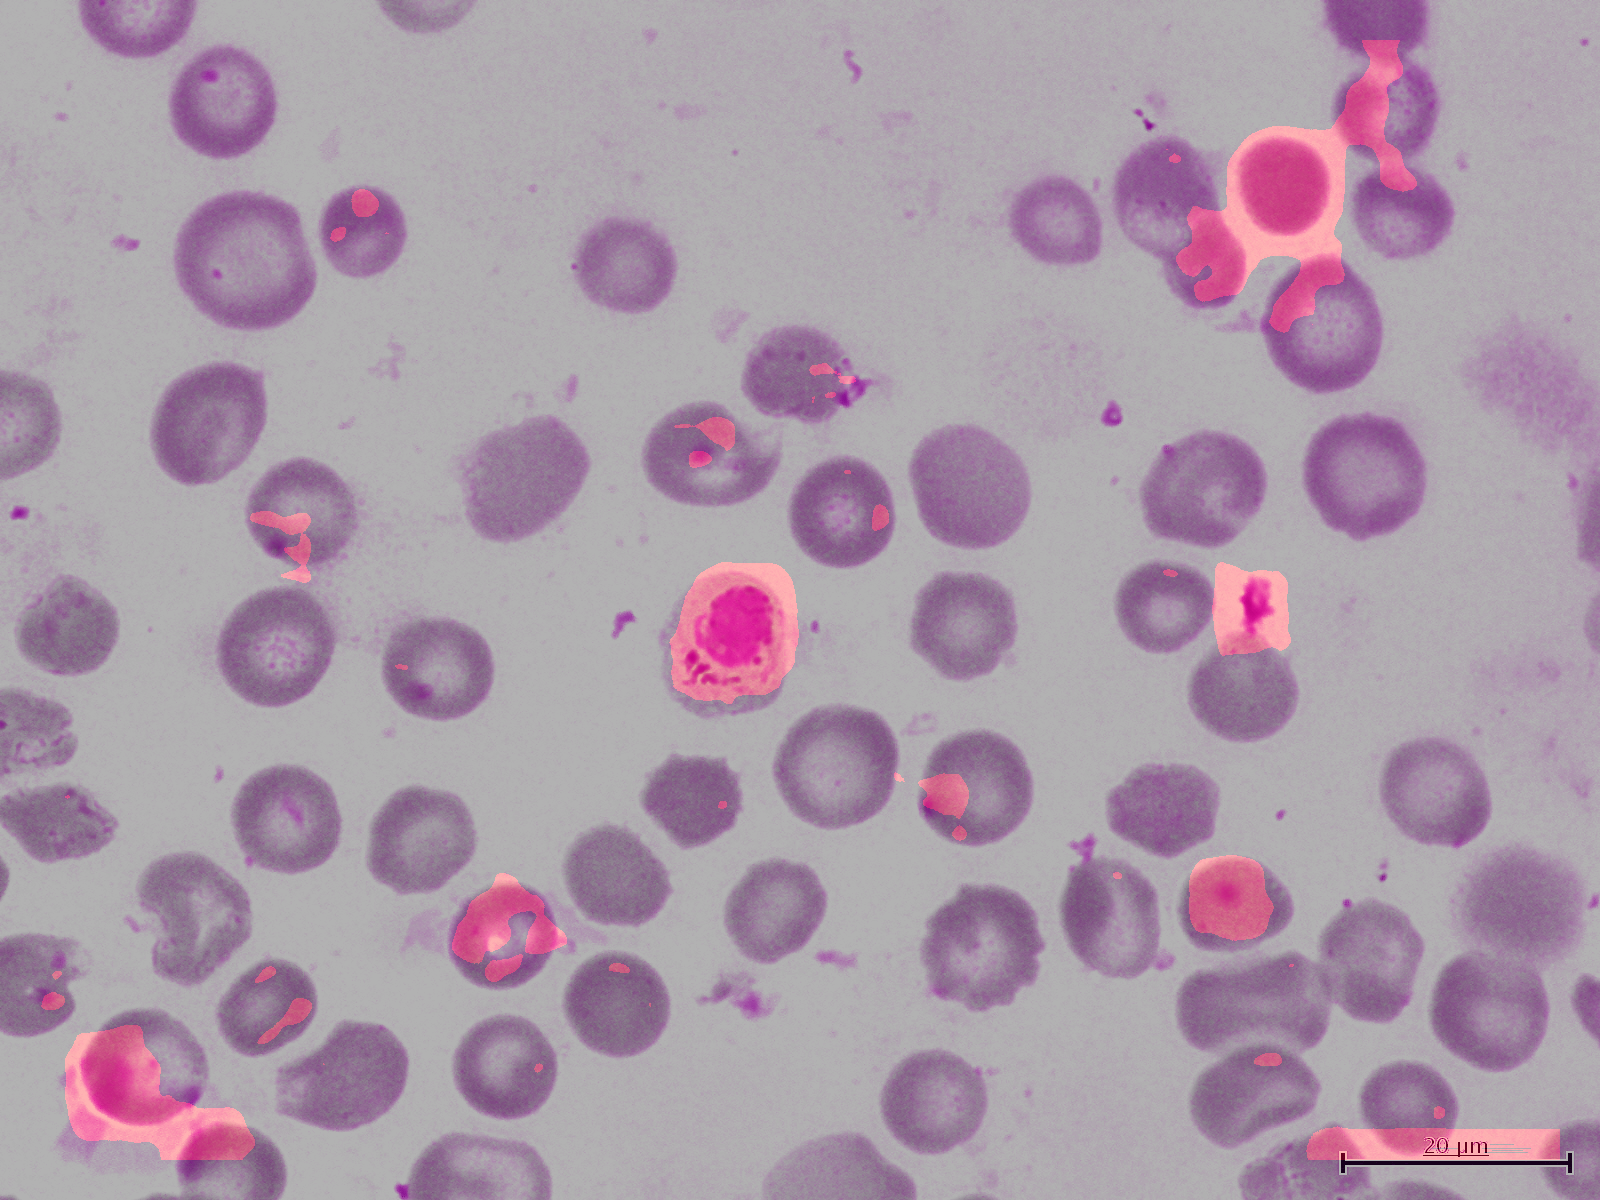
\includegraphics[width=\linewidth]{images/macenko_0a747cb3-c720-4572-a661-ab5670a5c42e.png}
    \caption{Macenko}
    \end{subfigure} \hfill
    \begin{subfigure}{0.3\textwidth}
    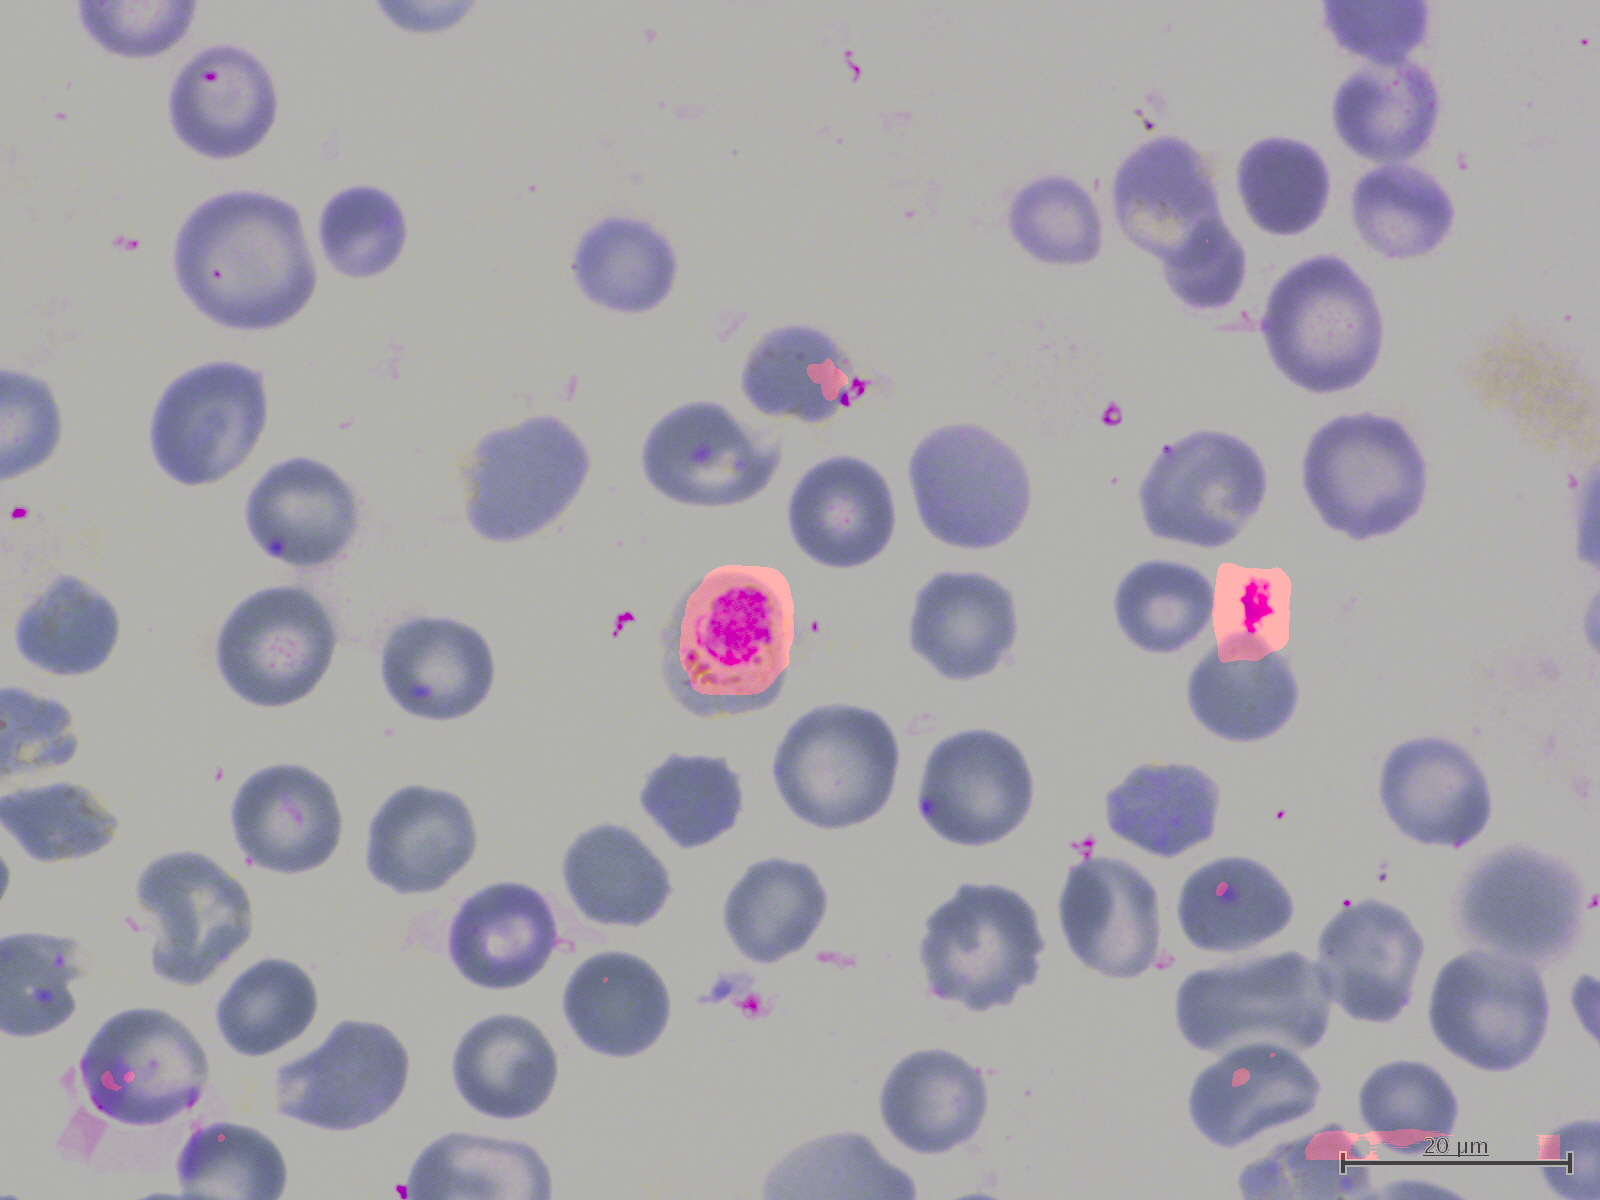
\includegraphics[width=\linewidth]{images/reinhard_0a747cb3-c720-4572-a661-ab5670a5c42e.png}
    \caption{Reinhard}
    \end{subfigure} \hfill
    \begin{subfigure}{0.3\textwidth}
    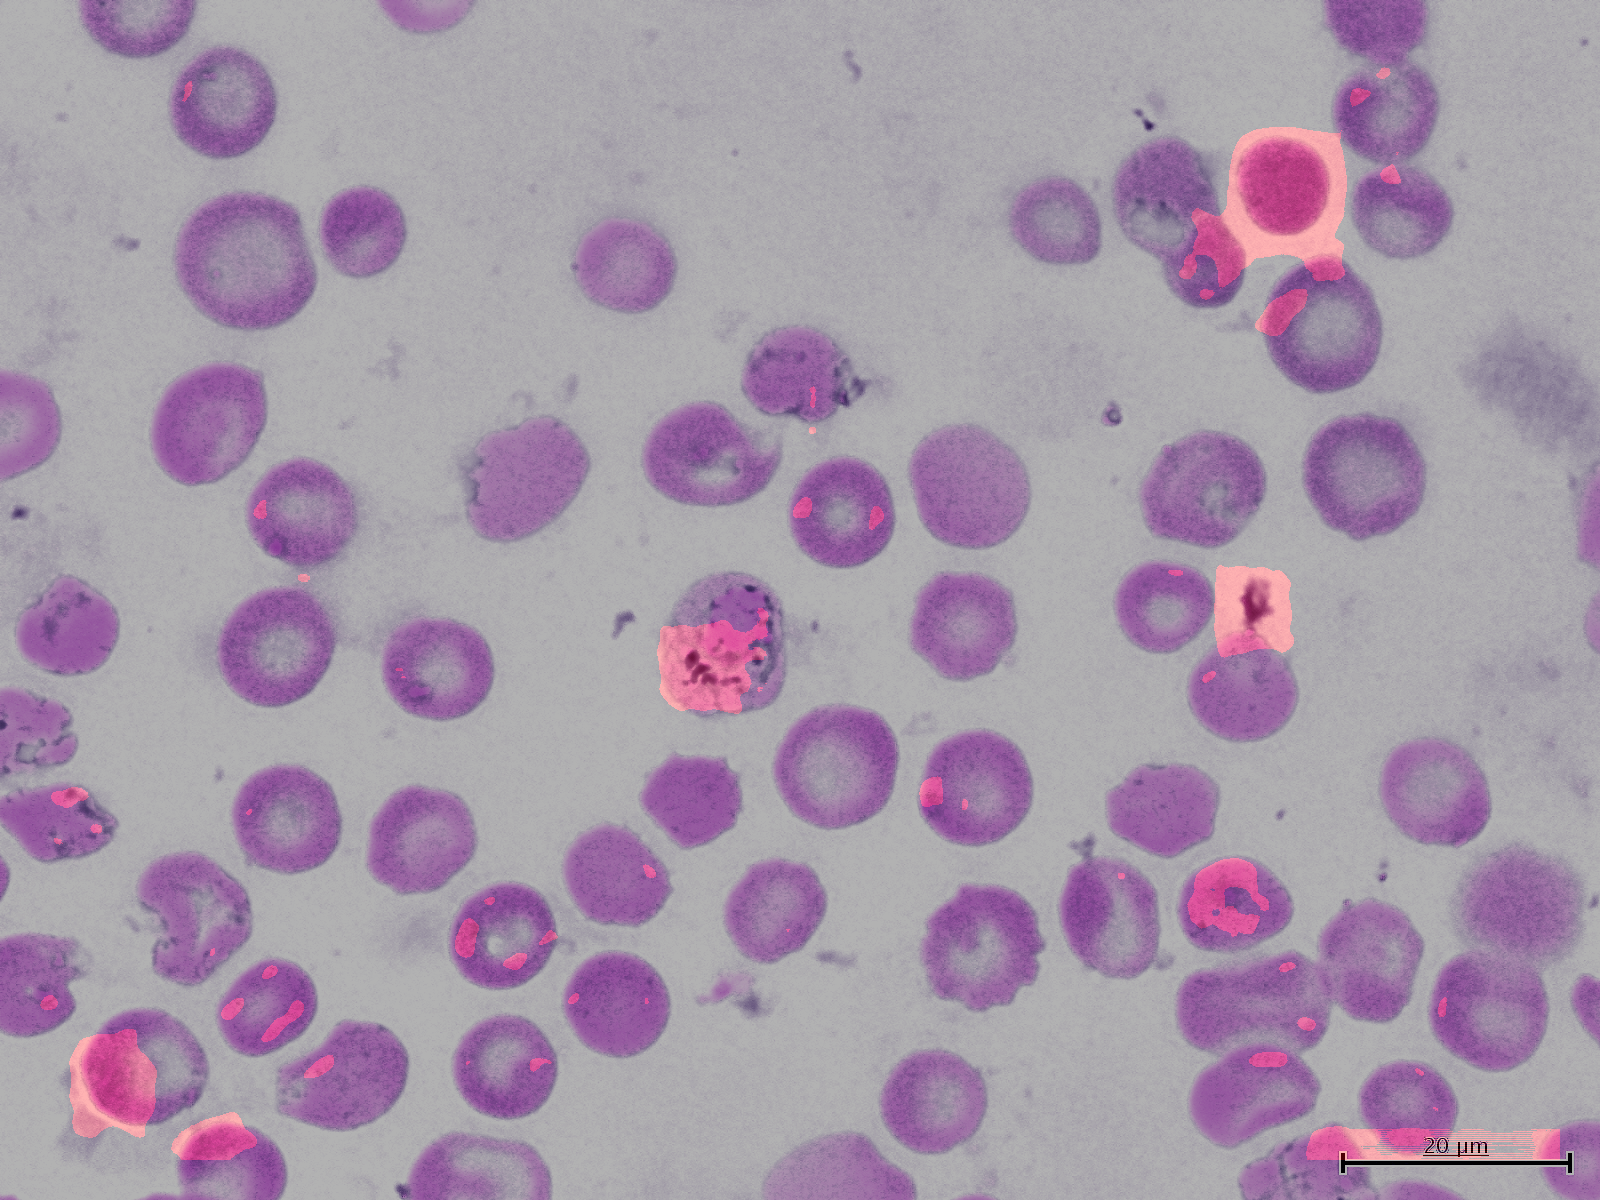
\includegraphics[width=\linewidth]{images/vahadane_0a747cb3-c720-4572-a661-ab5670a5c42e.png}
    \caption{Vahadane}
    \end{subfigure} \hfill
    \caption{Results of the LeNet model using different staining techniques}
\end{figure}

\begin{figure}
    \centering
    \begin{subfigure}{0.45\textwidth}
    \centering
    \includegraphics[width=\linewidth]{images/"Macenko_ True Positives vs False Negatives".png}
    % \caption{}
    % \label{fig:my_label}
    \end{subfigure} \hfill
    \begin{subfigure}{0.45\textwidth}
    \centering
    \includegraphics[width=\linewidth]{images/"Macenko_ True Positives vs False Positives".png}
    % \caption{}
    % \label{fig:my_label}
    \end{subfigure}
    \caption{Macenko Analysis Curves}
    \label{fig:macenko_curves}
\end{figure}

\begin{figure}
    \centering
    \begin{subfigure}{0.45\textwidth}
    \centering
    \includegraphics[width=\linewidth]{images/"Reinhard_ True Positives vs False Negatives".png}
    % \caption{}
    % \label{fig:my_label}
    \end{subfigure} \hfill
    \begin{subfigure}{0.45\textwidth}
    \centering
    \includegraphics[width=\linewidth]{images/"Reinhard_ True Positives vs False Positives".png}
    % \caption{}
    % \label{fig:my_label}
    \end{subfigure}
    \caption{Reinhard Analysis Curves}
    \label{fig:macenko_curves}
\end{figure}

\begin{figure}
    \centering
    \begin{subfigure}{0.45\textwidth}
    \centering
    \includegraphics[width=\linewidth]{images/"Vahadane_ True Positives vs False Negatives".png}
    % \caption{}
    % \label{fig:my_label}
    \end{subfigure} \hfill
    \begin{subfigure}{0.45\textwidth}
    \centering
    \includegraphics[width=\linewidth]{images/"Vahadane_ True Positives vs False Positives".png}
    % \caption{}
    % \label{fig:my_label}
    \end{subfigure}
    \caption{Vahadane Analysis Curves}
    \label{fig:macenko_curves}
\end{figure}

    
% \subsection{Results and Analysis}
    

    
    % \clearpage
    
    \section{Conclusion and Future Work}
    In this report, the results of the patch-based LeNet architecture for the task of semantic segmentation of Malaria Cells in Thin Blood Films is presented. The results under different stain normalization techniques were compared and the one under Vahadane et al.\cite{vahadane} were found to be the best. 

    \clearpage
    
    \bibliography{major_project}
    \bibliographystyle{unsrtnat}
    
\end{document}